\documentclass[crop,tikz]{standalone} 
\usepackage{tikz, amsmath, amssymb, graphicx} 

\DeclareMathAlphabet\mathbfcal{OMS}{cmsy}{b}{n}

\newcommand{\Mt}{\mathbfcal{M}}
\newcommand{\Yt}{\mathbfcal{Y}}
\newcommand{\Ft}{\mathbfcal{F}}

\usetikzlibrary{positioning, shapes.geometric} 

\begin{document}  

\tikzset{fontscale/.style = {font=\relsize{#1}}
    }

\begin{tikzpicture} 

 
\node[inner sep=0pt] at (0, 0) {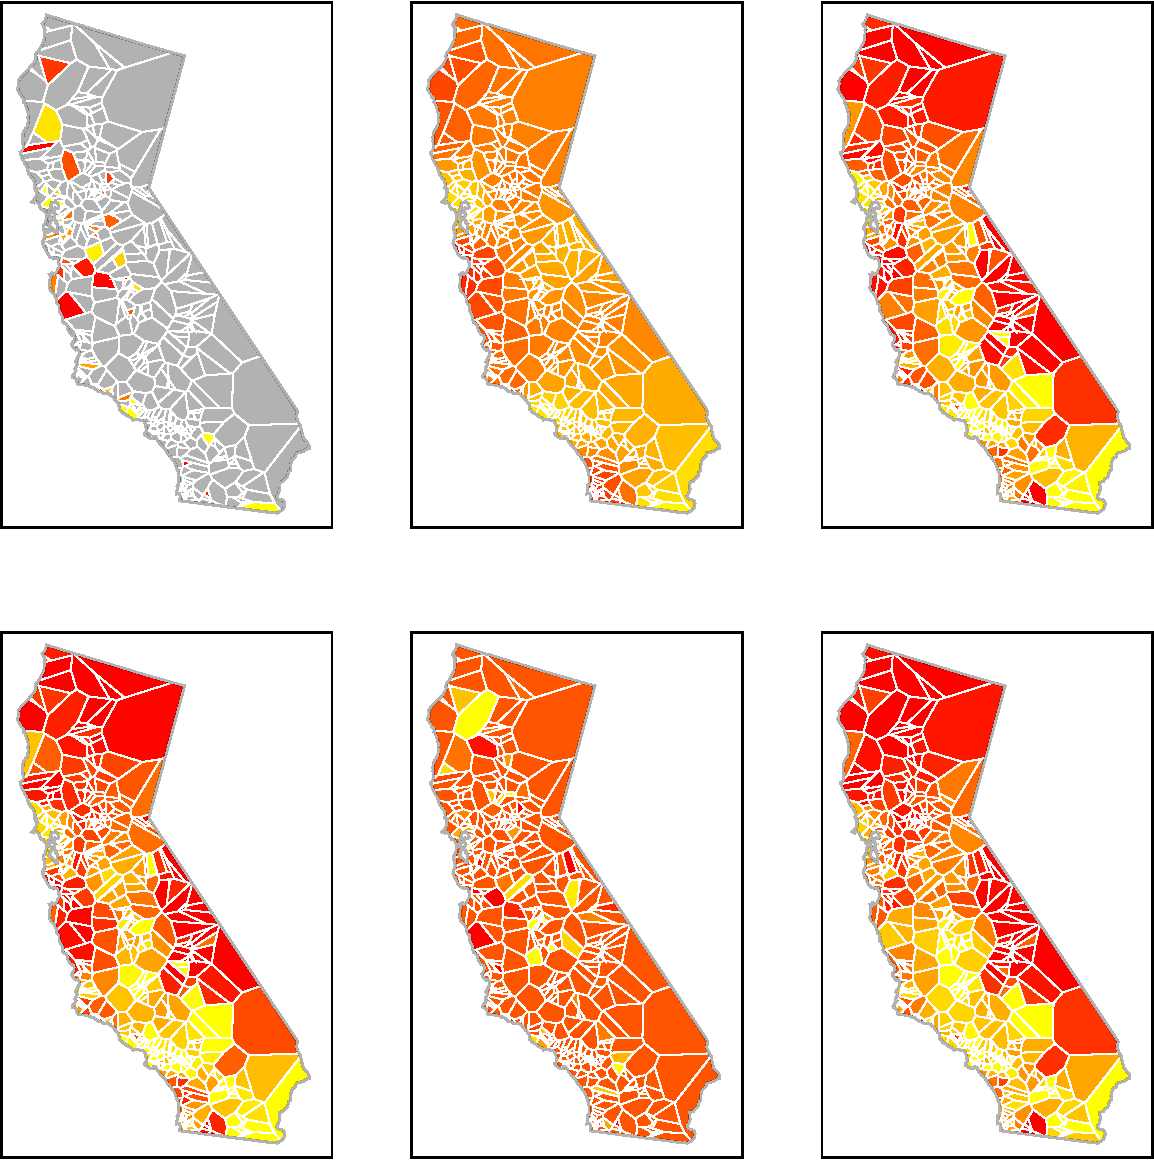
\includegraphics[width=.4\textwidth]{cali_preds_plot.pdf}};

\node[inner sep=0pt, scale=0.4] at (-1.73, 2.6) {Ground truth};
\node[inner sep=0pt, scale=0.4] at (0, 2.6) {KGR};
\node[inner sep=0pt, scale=0.4] at (1.73, 2.6) {RNC};
\node[inner sep=0pt, scale=0.4] at (-1.73, -0.1) {KG-RNC};
\node[inner sep=0pt, scale=0.4] at (0, -0.1) {Ridge (global)};
\node[inner sep=0pt, scale=0.4] at (1.73, -0.1) {Ridge (local)};

\end{tikzpicture}
\end{document} 